% Originally: content/week-10.tex, \section{Vector calculus operators} (Corsin Week 10)

\section{Vector calculus operators}
\label{sec:vector_calculus_operators}

\begin{definition}[Vector field]
\label{def:vector_field}
Let $U \subseteq \mathbb{R}^n$ be open. A \newterm{$C^k$ vector field} (\germanterm{Vektorfeld}) is a function $F : U \to \mathbb{R}^n$ of class $C^k(U,\mathbb{R}^n)$.
The scalar functions $F_1, \dots, F_n$ in $F(x) = (F_1(x), \dots, F_n(x))\transp$ are called the \newterm{components}.
\end{definition}

\begin{definition}[Gradient]
\label{def:gradient_vector_field}
Let $f : U \to \mathbb{R}$ be a function of class $C^k$ on an open set $U \subseteq \mathbb{R}^n$. The \newterm{gradient} of $f$ is the $C^{k-1}$ vector field
\[\operatorname{grad} f(x) = \nabla f(x) := \begin{pmatrix} \partial_1 f(x) \\ \vdots \\ \partial_n f(x) \end{pmatrix}.\]
\end{definition}

\begin{definition}[Divergence]
\label{def:divergence}
For a $C^1$ vector field $F : U \to \mathbb{R}^n$, the \newterm{divergence} is the scalar function
\[\divg F(x) := \sum_{i=1}^n \partial_i F_i(x).\]
In 3D, physicists write this as $\vec{\nabla} \cdot \vec{F}(x) = \partial_1 F_1(x) + \partial_2 F_2(x) + \partial_3 F_3(x)$.
\end{definition}

\begin{ainote}
Intuitively, $\divg F(x)$ tells us how much flow of $F$ is generated at $x$. If $\divg F(x) = 0$, then the total generated flow is zero.
If $\divg F(x) > 0$, then $x$ is a \newterm{source} (\germanterm{Quelle}), meaning more flow is generated than removed.
If $\divg F(x) < 0$, then $x$ is a \newterm{sink} (\germanterm{Senke}), meaning more flow is removed than generated.

% Supplement: Sascha Brack/Class Notes/Week_10_Notes_Monday.pdf, p. 9
\begin{center}
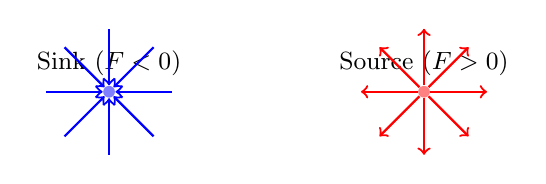
\begin{tikzpicture}[scale=1]
  \node[circle, fill=blue!50, inner sep=1.5pt, label=above:{\small Sink ($\divg F < 0$)}] (sink) at (0,0) {};
  \foreach \angle in {0,45,...,315} {
    \draw[blue, thick, <-] (sink) -- ++(\angle:0.8);
  }
  
  \node[circle, fill=red!50, inner sep=1.5pt, label=above:{\small Source ($\divg F > 0$)}] (source) at (4,0) {};
  \foreach \angle in {0,45,...,315} {
    \draw[red, thick, ->] (source) -- ++(\angle:0.8);
  }
\end{tikzpicture}
\end{center}
\end{ainote}

\begin{definition}[Rotation/Curl]
\label{def:rotation}
Let $F$ be a $C^k$ vector field on an open set $U \subseteq \mathbb{R}^3$. The \newterm{rotation} or \newterm{curl} of $F$ is the $C^{k-1}$ vector field
\[\curl F(x) := \begin{pmatrix} \partial_2 F_3(x) - \partial_3 F_2(x) \\ \partial_3 F_1(x) - \partial_1 F_3(x) \\ \partial_1 F_2(x) - \partial_2 F_1(x) \end{pmatrix}.\]
Physicists write $\curl F(x) = \vec{\nabla} \times \vec{F}(x)$.
In $\mathbb{R}^2$, the rotation of a vector field $F = (F_1, F_2)\transp$ is the scalar function $\curl F(x) := \partial_1 F_2(x) - \partial_2 F_1(x)$.
\end{definition}

\begin{ainote}
Intuitively, $\curl F(x)$ tells us how much the field tends to rotate around $x$. If $\curl F(x) \neq 0$, a small wheel centered at $x$ would rotate.

% Supplement: Sascha Brack/Class Notes/Week_10_Notes_Monday.pdf, p. 10
\begin{center}
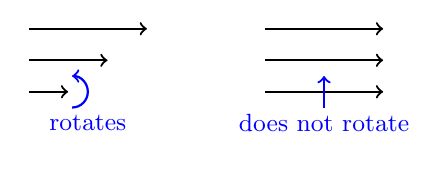
\begin{tikzpicture}[scale=1]
  % Rotates
  \draw[thick, ->] (0, 0.4) -- (1.5, 0.4);
  \draw[thick, ->] (0, 0) -- (1.0, 0);
  \draw[thick, ->] (0, -0.4) -- (0.5, -0.4);
  \node[blue, font=\small] at (0.75, -0.8) {rotates};
  \draw[blue, thick, ->] (0.55,-0.6) arc (-90:90:0.2);
  
  % Does not rotate
  \draw[thick, ->] (3, 0.4) -- (4.5, 0.4);
  \draw[thick, ->] (3, 0) -- (4.5, 0);
  \draw[thick, ->] (3, -0.4) -- (4.5, -0.4);
  \node[blue, font=\small] at (3.75, -0.8) {does not rotate};
  \draw[blue, thick, ->] (3.75,-0.6) -- (3.75,-0.2);
\end{tikzpicture}
\end{center}
\end{ainote}

\begin{example}[Computing vector calculus operators]
\label{ex:compute_operators}
Given $\phi : \mathbb{R}^3 \to \mathbb{R}$, $\phi(x,y,z) := x^2 + y^2 + z^2 e^{-xy}$.
Let us compute the gradient, the divergence of the gradient, and the rotation of the gradient.
\begin{itemize}
    \item \textbf{Gradient:}
    \[\nabla \phi(x,y,z) = \begin{pmatrix} 2x - yz^2 e^{-xy} \\ 2y - xz^2 e^{-xy} \\ 2z e^{-xy} \end{pmatrix}.\]
    
    \item \textbf{Divergence of the gradient} (denoted $\divg(\nabla \phi)$ or $\Delta \phi$):
    \begin{align*}
    \divg(\nabla \phi) &= \partial_x(2x - yz^2 e^{-xy}) + \partial_y(2y - xz^2 e^{-xy}) + \partial_z(2z e^{-xy}) \\
    &= (2 + y^2 z^2 e^{-xy}) + (2 + x^2 z^2 e^{-xy}) + (2 e^{-xy}) \\
    &= 4 + (x^2 z^2 + y^2 z^2 + 2) e^{-xy}.
    \end{align*}
    
    \item \textbf{Rotation of the gradient} ($\curl(\nabla \phi)$):
    \begin{align*}
    \curl(\nabla \phi) &= \begin{pmatrix} \partial_y(2z e^{-xy}) - \partial_z(2y - xz^2 e^{-xy}) \\ \partial_z(2x - yz^2 e^{-xy}) - \partial_x(2z e^{-xy}) \\ \partial_x(2y - xz^2 e^{-xy}) - \partial_y(2x - yz^2 e^{-xy}) \end{pmatrix} \\
    &= \begin{pmatrix} -2xz e^{-xy} - (-2xz e^{-xy}) \\ -2yz e^{-xy} - (-2yz e^{-xy}) \\ -z^2 e^{-xy} - (-z^2 e^{-xy}) \end{pmatrix} = \begin{pmatrix} 0 \\ 0 \\ 0 \end{pmatrix}.
    \end{align*}
    This is not a coincidence: for any $C^2$ function $f$, $\curl(\nabla f) = 0$ by Schwarz's theorem.
\end{itemize}
\end{example}

% Supplement: Analysis_II_Script_v1.pdf, p. 163
\begin{exercise}[$\curl\circ\grad=0$ and $\divg\circ\curl=0$]
\label{ex:curl_grad_div_curl_zero}
Let $f$ be a twice continuously differentiable function and $F$ a twice continuously
differentiable vector field on an open set $U \subseteq \mathbb{R}^3$. Show that
\[\curl(\grad f) = 0 \qquad\text{and}\qquad \divg(\curl F) = 0.\]
\end{exercise}

\begin{exercisesolution}[Proof of \cref{ex:curl_grad_div_curl_zero}]
% Generator: Claude Sonnet 5 (High)
Both identities follow from Schwarz's theorem (\cref{thm:schwarz_mixed_partials}), which
applies since $f,F \in C^2$.

\textbf{$\curl(\grad f)=0$.} The first component of $\curl(\grad f)$ is
$\partial_2(\partial_3f) - \partial_3(\partial_2f) = 0$ by Schwarz, and the other two
components vanish the same way, cyclically permuting the indices. This is exactly
\cref{ex:compute_operators}'s observation above, now stated and proved in general.

\textbf{$\divg(\curl F)=0$.}
\[\divg(\curl F) = \partial_1(\partial_2F_3-\partial_3F_2) + \partial_2(\partial_3F_1-\partial_1F_3)
  + \partial_3(\partial_1F_2-\partial_2F_1),\]
and every one of the six terms cancels against another by Schwarz: $\partial_1\partial_2F_3$
cancels $-\partial_2\partial_1F_3$, $-\partial_1\partial_3F_2$ cancels
$\partial_3\partial_1F_2$, and $\partial_2\partial_3F_1$ cancels $-\partial_3\partial_2F_1$.
\end{exercisesolution}

\begin{remark}
This is the classical-vector-calculus shadow of \qt{$d^2=0$}
(\cref{thm:exterior_derivative}\textbf{(2)}, \cref{ch:differential_forms}): $\grad$, $\curl$ and
$\divg$ are exactly the $0$-, $1$- and $2$-form incarnations of the exterior derivative in
$\mathbb{R}^3$ (\cref{ex:exterior_derivative_gradient_curl}), and both identities above are the
single fact $d\circ d=0$ read off once in each degree.
\end{remark}

% Supplement: Analysis_II_Script_v1.pdf, p. 164
\begin{proposition}[Product rule for the curl]
\label{prop:curl_product_rule}
Let $U \subseteq \mathbb{R}^3$ be open, $F : U \to \mathbb{R}^3$ a $C^1$ vector field, and
$\varphi : U \to \mathbb{R}$ a $C^1$ function. Then
\[\curl(\varphi F) = \varphi\,\curl(F) + (\grad\varphi)\times F.\]
\end{proposition}

\begin{proof}
By the product rule applied componentwise, e.g.\ for the first component,
\[\partial_2(\varphi F_3) - \partial_3(\varphi F_2)
  = \varphi(\partial_2F_3-\partial_3F_2) + (\partial_2\varphi)F_3 - (\partial_3\varphi)F_2,\]
and the first term is $\varphi\,\curl(F)$'s first component, the last two are
$((\grad\varphi)\times F)$'s first component. The other two components follow identically,
cyclically permuting the indices.
\end{proof}

\begin{ainote}
The official script sets this identity as an exercise (Ex.\ 14.61) but states it without the
first term, as $\curl(\varphi F) = (\grad\varphi)\times F$ --- which is false in general: taking
$\varphi\equiv1$ would force $\curl F \equiv 0$ for every $F$. The missing term is exactly
$\varphi\,\curl(F)$, restored above. (The script's exercise also names the vector field $f$ in
its statement and $F$ in its conclusion, as though the two were interchangeable.)
\end{ainote}


% --- exercises relocated here from the dissolved sheets ---

% Originally: content/week-11.tex, \exercisesheet{11}, problem 11.1
% Source: exercises/Ex11_Analysis2_eng.pdf

\begin{exercise}[11.1 --- Flow of vector field \textnormal{(important)}]
\label{ex:11.1}
Compute the flow of the vector field
\[V : (x,y,z) \mapsto (x,y,z-x^2-y^2)\]
through the upper hemisphere $S = \{(x,y,z)\in\mathbb{R}^3 : x^2+y^2+z^2=1,\ z\geq0\}$ from
\qt{inside} to \qt{outside}. That is the number
\[\int_S V(x)\cdot\nu(x)\,d\vol_2.\]
\end{exercise}

% Source: exercises/Ex11_Analysis2_eng.pdf, p. 2
